\documentclass[12pt]{article}

\usepackage[numbers, compress]{natbib}
\usepackage[utf8]{inputenc} % allow utf-8 input
\usepackage{hyperref}       % hyperlinks
\usepackage{url}            % simple URL typesetting
\usepackage{booktabs}       % professional-quality tables
\usepackage{amsfonts}       % blackboard math symbols
\usepackage{nicefrac}       % compact symbols for 1/2, etc.
\usepackage{microtype}      % microtypography
\usepackage{xcolor}         % colors
\usepackage{tikz}
\usetikzlibrary{arrows}
\usepackage{amsmath}
\usepackage{mathtools}
\usepackage{bbm}
\usepackage{amssymb}
\usepackage{algorithm}
\usepackage{algpseudocode}
\usepackage{caption}
\usepackage{subcaption}
\usepackage{graphicx}
\usepackage{float}
\usepackage{placeins}
\usepackage{enumitem}
\usepackage[margin=1in]{geometry}
\usepackage{pdfpages}
\usepackage{setspace}
\onehalfspacing
\setlength\parskip{0.8em plus 0.1em minus 0.1em}
\setlength\parindent{0pt}

%images
\graphicspath{{./img/}}


%bibliography
\bibliographystyle{plainnat}


\begin{document}
	
	\pagenumbering{gobble}
	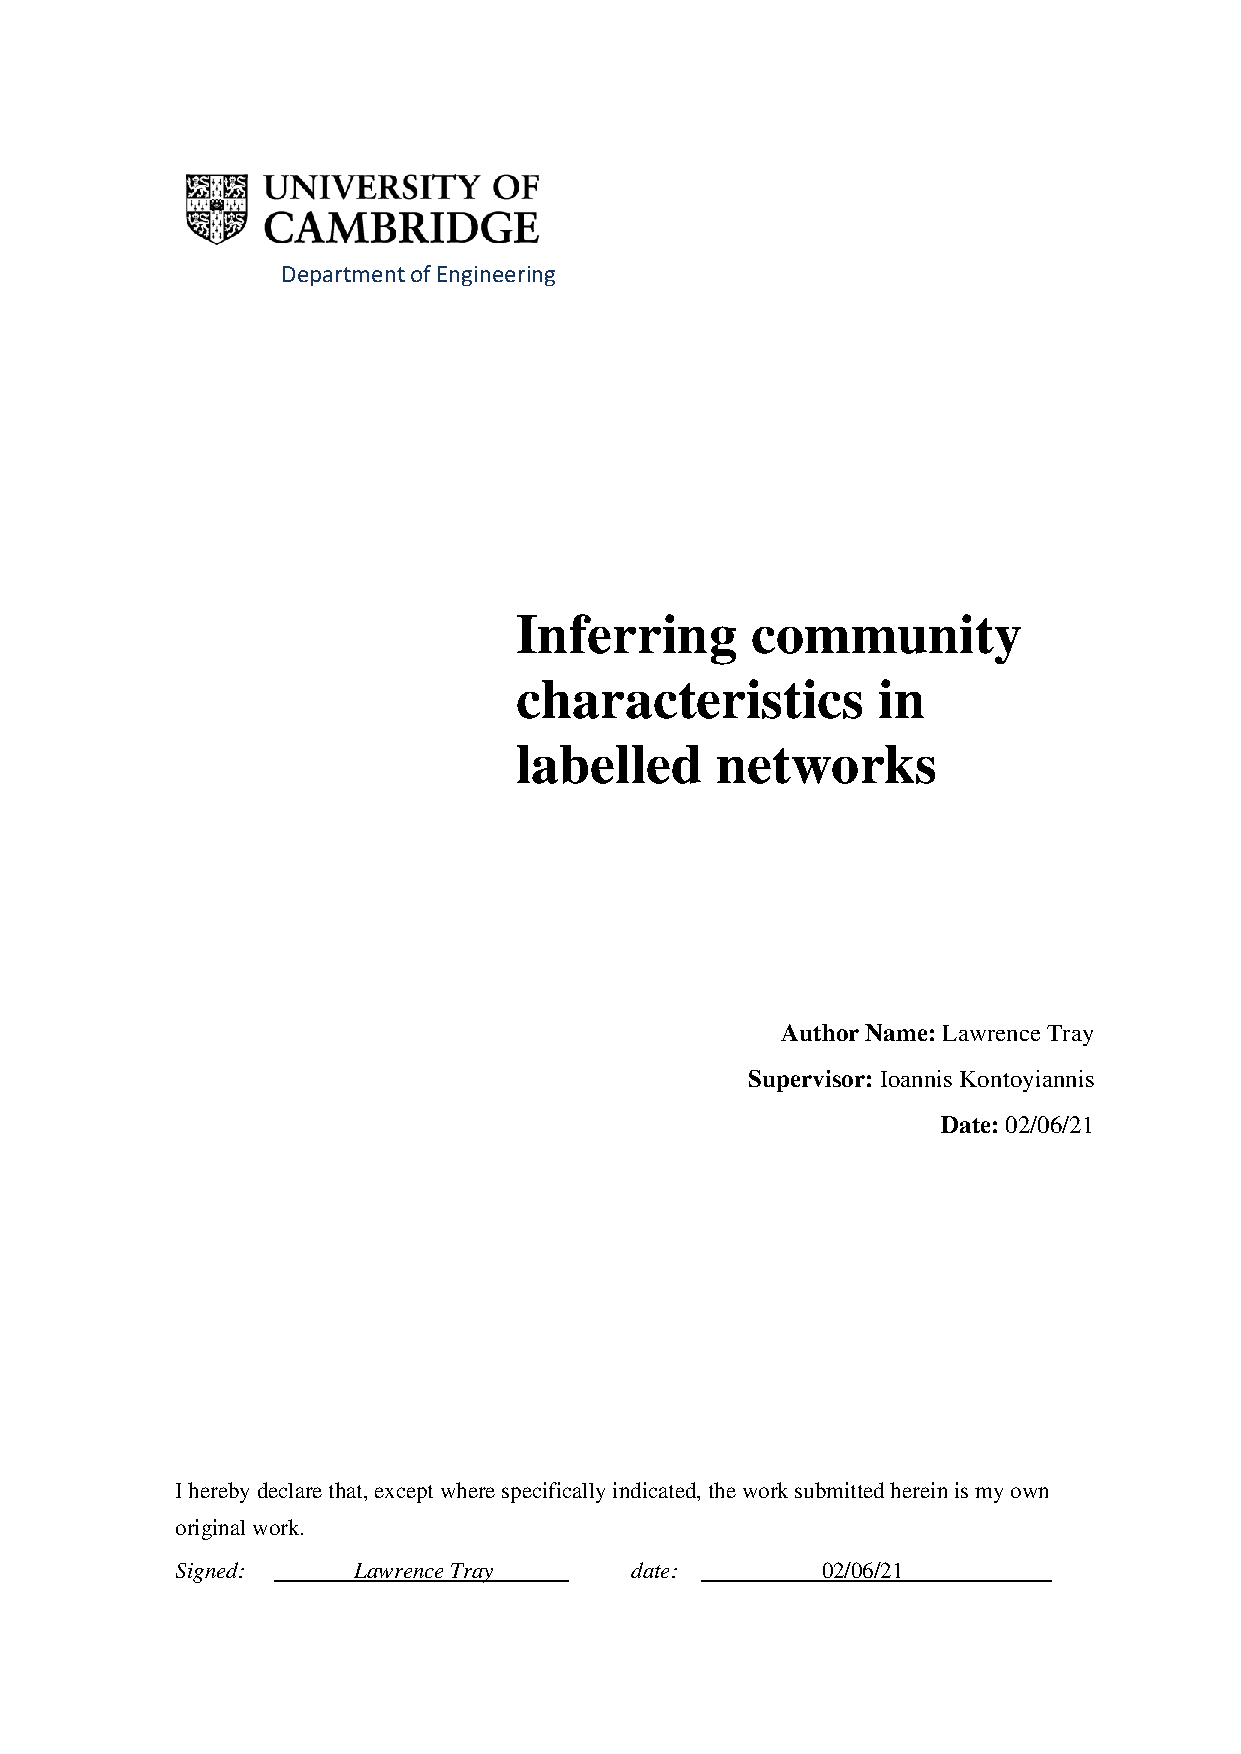
\includepdf{coversheet}
	\pagenumbering{arabic}
	
	%
	\section*{Technical Abstract}
	Labelled networks form a very common and important class of data,
	naturally appearing in numerous applications in science and engineering.
	A typical inference goal is to determine how the vertex labels
	(called features) affect the network's graph structure. A standard
	approach has been to partition the network into blocks grouped
	by distinct values of the feature of interest. A block-based random
	graph model -- typically a variant of the stochastic block model (SBM) --
	is then used to test for evidence of asymmetric behaviour within these
	feature-based communities. Nevertheless, the resulting communities
	often do not produce a natural partition of the graph. In this work
	we introduce a new generative model, the feature-first block model (FFBM),
	which is more effective at describing vertex-labelled undirected
	graphs and also facilitates the use of richer queries on labelled networks.
	We develop a Bayesian framework for inference with this model,
	and we present a method to efficiently sample from the posterior
	distribution of the FFBM parameters. The FFBM's structure is kept
	deliberately simple to retain easy interpretability of the parameter
	values. We apply the proposed methods to a variety of network data
	to extract the most important features along which the vertices
	are partitioned. The main advantages of the proposed approach are
	that the whole feature-space is used automatically, and features
	can be rank-ordered implicitly according to impact. Any features
	that do not significantly impact the high-level structure can be
	discarded to reduce the problem dimension. In cases where the vertex
	features available do not readily explain the community structure
	in the resulting network, the approach detects this and is protected
	against over-fitting. Results on several real-world datasets
	illustrate the performance of the proposed methods. 
	
\end{document}
